% !TEX root = ./main.tex

\section{Linear Maps}

\subsection{Vector Space of Linear Maps}

Now, we may need more vector spaces, so let $V$ AND $W$ denoting vector spaces
over $\F$.

\begin{definition} [$\Polys{\F}{\empty}$]
    $\Polys{\F}{\empty}$ is the vector space of all polynomials with coefficients in $\F$.
\end{definition}

\begin{definition} [Linear Map]
   A \textbf{linear map} from $V$ to $W$ is a function
   $T : V \to W$ with the following properties:
   \begin{itemize}
       \item additivity: $T(u_1 + u_2) = Tu_1 + Tu_2$ for all $u_1, u_2 \in V$
       \item homogeneity: $T(\lambda u) = \lambda(Tu)$ for all $\lambda \in \F$ and all $u \in V$
   \end{itemize}
\end{definition}

For linear maps, we often use the
notation $Tu$ as well as the more standard functional notation
$T(u)$.

\begin{definition} [$\Lin{V, W}$]
   The set of all linear maps from $V$ to $W$ is denoted
   $\Lin{V, W}$. 
\end{definition}

\begin{example} Examples of Linear Maps:
   \begin{itemize}
       \item Zero: Define $0 \in \Lin{V,W}$ by $0u = 0$ for all $u \in V$.
       \item Identity map: Define $I \in \Lin{V,V}$ by $Iu = u$ for all $u \in V$.
       \item Differentiation: Define $D \in \Lin{\Polys{\R}{\empty}, \Polys{\R}{\empty}}$ by $Dp = p'$.
       \item Integration: Define $T \in \Lin{\Polys{\R}{\empty}, \R}$ by $Tp = \int_0^1 p(x) \dd{x}$.
       \item Multiplication by $x^2$: Define $T \in \Lin{\Polys{\R}{\empty}, \Polys{\R}{\empty}}$ by
       \[ (Tp)(x) = x^2 p(x) \]
       for $x \in \R$.
       \item Backward shift: Define $T \in \Lin{\F^{\infty}, \F^{\infty}}$ by
       \[ T(x_1, x_2, x_3, \dots) = (x_2, x_3, \dots). \]
       \item From $\R^3$ to $\R^2$: Define $T \in \Lin{\R^3, \R^2}$ by
       \[ T(x, y, z) = (2x - y + 3z, 7x + 5y - 6z). \]
   \end{itemize} 
\end{example}

\begin{theorem}
    Suppose $\listofvectors$ is a basis of $V$ and $\listofnames{w}{n} \in W$. Then there
    exists a unique linear map $T : V \to W$ such that
    \[ Tv_j = w_j \]
    for each $j = 1, \dots, n$.

    \begin{proof*}
        Define $T: V \to W$ by
        \[ T(\linearcombination) = a_1w_1 + \dots + a_nw_n, \]
        where $\listofscalars$ are arbitrary elements of $\F$.

        It is straightforward to check the above map is additive, just take all the
        coefficients except $a_i$ to be 0. The distributive property handles homogeneity.

        There cannot be another such map because if you add all the constraints
        together, you get precisely this relation. \qed
    \end{proof*}
\end{theorem}

\begin{definition} [Addition and Scalar Multiplication on $\Lin{V, W}$]
   Suppose $S, T \in \Lin{V, W}$ and $\lambda \in \F$. The sum $S+T$ is defined as:
   \[ (S+T)(u) = Su + Tu \]
    and the product $\lambda T$ is defined as:
    \[ (\lambda T)(u) = \lambda (Tu) \]
    for all $u \in V$.

    Clearly, these maps are also linear maps, thus stay in the set.
\end{definition}

\begin{note} [$\Lin{V, W}$ is a Vector Space]
   With the operations of addition and scalar multiplication as defined above, $\Lin{V, W}$
   is a vector space. 
\end{note}

\begin{definition} [Product of Linear Maps]
   If $T \in \Lin{U, V}$ and $S \in \Lin{V, W}$, then the product $ST \in \Lin{U, W}$ is defined by
   \[ (ST)(u) = S(Tu) \]
   for $u \in U$.
\end{definition}

\begin{note} [Algebraic Properties of Products of Linear Maps]
   \begin{itemize}
       \item Associativity: $(T_1 T_2)T_3 = T_1(T_2 T_3)$
       \item Identity: $TI = IT = T$ (note this may be two different $I$'s)
       \item Distributive Properties: $(S_1 + S_2)T = S_1 T + S_2 T$ and $S(T_1 + T_2) = ST_1 + ST_2$
   \end{itemize} 
\end{note}

\begin{theorem} [Linear Maps take 0 to 0]
   Suppose $T$ is a linear map from $V$ to $W$. Then $T(0) = 0$. 
\end{theorem}

There's a tricky bit about the word "linear". In calculus, we say any
$f(x) = mx + b$, this is termed linear. However, in the sense of vector spaces,
this function is only linear if and only if $b = 0$.

\subsection{Null Spaces and Ranges}

\begin{definition} [Null Space]
   For $T \in \Lin{V, W}$, the \textbf{null space} of $T$, denoted $\null T$, is the subset of $V$
   containing those vectors that $T$ maps to 0:
   \[ \Null T = \{ u \in V : Tu = 0 \} \]
\end{definition}

\begin{example} Examples of Null Spaces:
   \begin{itemize}
      \item Suppose $T$ is the zero map form $V$ to $W$; in other words, $Tu = 0$ for
      every $u \in V$. Then $\Null T = V$.
      \item Suppose $\phi \in \Lin{\C^3, \C}$ is defined by $\phi(z_1, z_2, z_3) = z_1 + 2z_2 + 3z_3$.
      Then $\Null \phi = \{ (z_1, z_2, z_3) \in \C^3 : z_1 + 2z_2 + 3z_3 = 0 \}$.
      \item Consider $D$, the differentiation map. The only functions whose derivative equals zero
      is the constant functions. Thus, the null space is the set of all constant functions.
   \end{itemize}
\end{example}

\begin{theorem} [The Null Space is a Subspace]
   Suppose $T \in \Lin{V, W}$. Then $\Null T$ is a subspace of $V$.
\end{theorem}

\begin{definition} [Injective]
   A function $T : V \to W$ is called \textbf{injective} or \textbf{one-to-one} if
   $Tu = Tv$ implies $u = v$.
\end{definition}

\begin{theorem}
   Let $T \in \Lin{V, W}$. Then $T$ is injective if and only if $\Null T = 0$.
\end{theorem}

\begin{definition} [Range]
   For $T \in \Lin{V, W}$, the \textbf{range} of $T$ is the subset
   of $W$ consisting of those vectors that are of the form $Tu$ for some $u \in V$:
   \[ \range T = \{ Tu : u \in V \} \]
\end{definition}

\begin{example} Ranges:
   \begin{itemize}
      \item Suppose $T$ is the zero map from $V$ to $W$; in other words,
      $Tu = 0$ for every $u \in V$. Then $\range T = \{ 0 \}$.
      \item Suppose $T \in \Lin{\R^2, \R^3}$ is defined by $T(x,y) = (2x, 5y, x+y)$,
      then $\range T = \{ (2x, 5y, x+y) : x, y \in \R \}$. A basis of $\range{T}$ is $(2, 0, 1)$, $(0, 5, 1)$.
      \item Consider the differentiation map $D \in \Lin{\Polys{\R}{\empty},\Polys{\R}{\empty}}$. Since every polynomial $q \in \Polys{\R}{\empty}$
      has a polynomial $p \in \Polys{\R}{\empty}$ such that $p' = q$, the range of $D$ is $\Polys{\R}{\empty}$.
   \end{itemize}
\end{example}

\begin{theorem} [The Range is a Subspace]
   If $T \in \Lin{V, W}$, then $\range T$ is a subspace of $W$.
\end{theorem}

\begin{definition} [Surjective]
   A function $T : V \to W$ is called \textbf{surjective} or \textbf{onto}
   if its range equals $W$.
\end{definition}

\begin{theorem} [Fundamental Theorem of Linear Maps]
   Suppose $V$ is finite-dimensional and $T \in \Lin{V, W}$. Then
   \[ \dim V = \dim \Null T + \dim \range T. \]
   \begin{proof*}
      (Proof Sketch)

      Let $u_1, \dots, u_m$ be a basis of $\Null T$; thus $\dim \Null T = m$.

      The linear independent list $u_1, \dots u_m$ can be extended to a basis
      \[ \listofnames{u}{m}, \listofvectors \]

      Thus $\dim V = m + n$.
      To complete the proof, we need to show that $\dim \range T = n$. We do this by proving that $Tv_1, \dots, TV_n$
      is a basis of $\range T$. \qed
   \end{proof*}
\end{theorem}

\begin{theorem} [A Map to a Smaller Dimensional Space is Not Injective]
   Suppose $V$ and $W$ are finite-dimensional vector spaces such that
   $\dim V > \dim W$. Then no linear map from $V$ to $W$ is injective.
   \begin{proof*}
      Suppose $T \in \Lin{V, W}$. Because
      \[ \dim V = \dim \Null T + \dim \range T \]
      and
      \[ \dim V > \dim W \geq \dim \range T \]
      we have $\dim \Null T > 0$. Thus $T$ is not injective. \qed
   \end{proof*}
\end{theorem}

\begin{theorem} [A Map to a Larger Dimensional Space is Not Surjective]
   Suppose $V$ and $W$ are finite-dimensional vector spaces such that
   $\dim V < \dim W$. Then no linear map from $V$ to $W$ is surjective.

   \begin{proof*}
      Suppose $T \in \Lin{V, W}$. Because
      \[ \dim V = \dim \null T + \dim \range T \]
      we have
      \[ \dim \range T \leq \dim V < \dim W \]

      Thus, $T$ is not surjective. \qed
   \end{proof*}
\end{theorem}

Now we can use these results to prove some facts about a related
subject, the theory of systems of linear equations.

\begin{definition} [Homogenous Linear Equations]
   Fix positive integers $m$ and $n$ and let $A_{j, k} \in \F$ for
   $j = 1, \dots, m$ and $k = 1, \dots, n$. Consider
   the homogeneous system of linear equations
   \begin{align*}
      \sum_{k=1}^n A_{1,k}x_k &= 0 \\
      &\vdots
      \sum_{k=1}^n A_{m,k}x_k &= 0
   \end{align*}

   These are called homogenous because the constant terms are
   all 0.
\end{definition}

We wish to ask the following: do there exist solutions other than the
trivial solution, i.e. $x_1 = \dots = x_n = 0$?

Define $T: \F^n \to \F^m$ by
\[ T(x_1, \dots, x_n) = \qty(\sum_{k=1}^n A_{1,k}x_k, \dots, \sum_{k=1}^n A_{m,k}x_k) \]

The equation $T(x_1, \dots, x_n) = 0$ is the same as the homogeneous
system of linear equations above. This is asking if $\null T = 0$,
which is the same asking: is $T$ injecive?

Well, we know $T$ is not injective if $\dim \F^n > \dim \F^m$, in other words
if $n > m$, so we have the following result:

\begin{theorem} [Homogenous System of Linear Equations]
   A homogeneous system of linear equations with more
   variables than equations has nonzero solutions.
\end{theorem}

Now, let us talk about other types of systems of linear equations.

\begin{definition} [Inhomogenous Linear Equations]
   Fix positive integers $m$ and $n$ and let $A_{j, k} \in \F$ for
   $j = 1, \dots, m$ and $k = 1, \dots, n$. Consider
   the inhomogeneous system of linear equations
   \begin{align*}
      \sum_{k=1}^n A_{1,k}x_k &= c_1 \\
      &\vdots
      \sum_{k=1}^n A_{m,k}x_k &= c_m
   \end{align*}

   These are called inhomogenous because the constant terms are
   not all 0.
\end{definition}

Now we wonder the following:
is there some choice of $\listofnames{c}{m} \in \F$ such that
no solution exists?

Define $T: \F^n \to \F^m$ by

\[ T(x_1, \dots, x_n) = \qty(\sum{k=1}^n A_{1,k}x_k, \dots, \sum{k=1}^n A_{m, k}x_k) \]

The equation $T(x_1, \dots, x_n) = (\listofnames{c}{m})$ is the same
as the inhomogeneous system of linear equations above. This is the same
as asking: is $T$ surjective?

We know $T$ is not surjective if $m > n$ (similar to previous logic),
so we have the following result:

\begin{theorem} [Inhomogenous System of Linear Equations]
   An inhomogeneous system of linear equations with more equations
   than variables has no solution for some choice of
   constant terms.
\end{theorem}

\subsection{Matrices}

\begin{definition} [Matrix]
   Let $m$ and $n$ denote positive integers. An $m$-by-$n$ \textbf{matrix}
   $A$ is a rectangular array of elements of $\F$ with $m$ rows and $n$ columns:

   $A = \begin{pmatrix}
     A_{1,1} && \dots && A_{1,n} \\
     \vdots && \empty && \vdots \\
     A_{m,1} && \dots && A_{m,n} 
   \end{pmatrix}$

   The notation $A_{j,k}$ denotes the entry in row $j$, column $k$ of $A$.
\end{definition}

The first index refers to the row numbers and the second index
refers to column numbers.

Thus $A_{2,3}$ refers to the entry in the second row, third column of $A$.

\begin{definition} [Matrix of a Linear Map, $\Matof{T}$]
   Suppose $T \in \L{V,W}$ and $\listofvectors$ is a basis of $V$ and
   $\listofnames{w}{m}$ is a basis of $W$. The \textbf{matrix} of $T$ with respect
   to these bases is the $m$-by-$n$ matrix $\Matof{T}$ whose entries
   $A_{j, k}$ are defined by
   \[ Tv_k = A_{1, k}w_1 + \dots + A_{m,k}w_m \]

   If the bases are not clear from the context, then the notation
   \[ \mathcal{M}(T, (\listofvectors), (\listofnames{w}{m})) \]
   is used.
\end{definition}

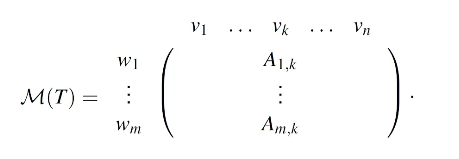
\includegraphics{matrix intuition.png}

To understand what the matrix really means, fix a column $k$
the $k$th column of $\Matof{T}$ consists of the scalars needed to write
\[ Tv_k = \sum_{j=1}^m A_{j,k}w_j.\]

The picture above should remind you that $Tv_k$ can be computed from
$\Matof{T}$ by multiplying each entry in the $k$th column by the corresponding
$w_j$ from the left column, and then adding up the resulting vectors.

\begin{example} [Matrices]
   Suppose $T \in \Lin{\F^2, \F^3}$ is defined by:
   \[ T(x,y) = (x+3y, 2x+5y, 7x+9y) \]
   Because $T(1, 0) = (1, 2, 7)$ and $T(0, 1) = (3, 5, 9)$, the matrix of
   $T$ with respect to the standard bases is the 3-by-2 matrix
   \[ \Matof{T} = \begin{pmatrix}
      1 & 3 \\
      2 & 5 \\
      7 & 9
   \end{pmatrix} \]

   Suppose $D \in \Lin{\Polys{\R}{3}, \Polys{\R}{2}}$ is the differentiation
   map. Beacuse $(x^n)' = nx^{n-1}$, the matrix of $D$ with respect
   to the standard bases of $\Polys{\R}{3}$ and $\Polys{\R}{2}$ is the
   3-by-4 matrix
   \[ \Matof{D} = \begin{pmatrix}
      0 & 1 & 0 & 0 \\
      0 & 0 & 2 & 0 \\
      0 & 0 & 0 & 3 \\
   \end{pmatrix}\]
\end{example}

Note that $\Matof{T}$ contains all the information about $T$.
The matrix contains all the information about how the
basis vectors transform under $T$, however, under linearity,
we can write every vector in $V$ as a linear combination of the basis
and since $T$ is linear we can see how any vector transforms.

\begin{definition} [Matrix Addition]
   The sum of two matrices of the same size is the matrix obtained
   by adding corresponding entries in the matrices:

   \[ \begin{pmatrix}
      A_{1,1} && \ldots && A_{1,n} \\
      \vdots && \empty && \vdots \\
      A_{m,1} && \dots && A_{m,n}
   \end{pmatrix}
   +
   \begin{pmatrix}
      C_{1,1} && \ldots && C_{1,n} \\
      \vdots && \empty && \vdots \\
      C_{m,1} && \dots && C_{m,n}
   \end{pmatrix} \]

   \[ = \begin{pmatrix}
      A_{1,1} + C_{1,1} && \ldots && A_{1,n} + C_{1,n}  \\
      \vdots && \empty && \vdots \\
      A_{m,1} + C_{m,1}  && \dots && A_{m,n} + C_{m,n}
   \end{pmatrix} \]
   
   In other words, $(A + C)_{j,k} = A_{j,k} + C_{j,k}$.
\end{definition}

In the following result, we assume that the same bases are used
for $\Matof{S+T}$, $\Matof{S}$, and $\Matof{T}$.

\begin{theorem} [Addition of Matrices]
   Suppose $S,T \in \Lin{V, W}$. Then $\Matof{S+T} = \Matof{S} + \Matof{T}$.
\end{theorem}

\begin{definition} [Scalar Multiplication of a Matrix]
   The produce of a scalar and a matrix is the matrix
   obtained by multiplying each entry in the matrix by the scalar:
   \[ \lambda \begin{pmatrix}
      A_{1,1} && \ldots && A_{1,n} \\
      \vdots && \empty && \vdots \\
      A_{m,1} && \dots && A_{m,n}
   \end{pmatrix}
   =
   \begin{pmatrix}
      \lambda A_{1,1} && \ldots && \lambda A_{1,n} \\
      \vdots && \empty && \vdots \\
      \lambda A_{m,1} && \dots && \lambda A_{m,n}
   \end{pmatrix}
   \]

   In other words, $(\lambda A)_{j,k} = \lambda A_{j,k}$.
\end{definition}

In the following result, we assume that the same bases are used
for $\Matof{\lambda T}$ and $\Matof{T}$.

\begin{theorem} [The Matrix of a Scalar Times a Linear Map]
   Suppose $\lambda \in \F$ and $T \in \Lin{V, W}$. Then
   $\Matof{\lambda T} = \lambda \Matof{T}$.
\end{theorem}

\begin{note} [$\F^{m,n}$]
   For $m$ and $n$ positive integers, the set of all $m$-by-$n$ matrices
   with entries in $\F$ is denoted by $\F^{m,n}$.
\end{note}

\begin{theorem} [$\dim \F^{m,n} = mn$]
   Suppose $m$ and $n$ are positive integers. With addition and scalar
   multiplication defined as above, $\F^{m, n}$ is a vector space with dimension
   $mn$.
\end{theorem}

Now we want to define matrix multiplication.

Consider the following vector spaces:
\begin{itemize}
   \item $V$ with basis $\listofvectors$.
   \item $W$ with basis $\listofnames{w}{m}$.
   \item $U$ with basis $\listofnames{u}{p}$.
\end{itemize}

Consider linear maps $T: U \to V$ and $S: V \to W$. We
want to define matrix multiplication such that
\[ \Matof{ST} = \Matof{S}\Matof{T} \]

We can try $(AB)_{j,k} = A_{j_k} \times B_{j,k}$, however
this will not line up with our definition for linear maps.

Instead consider the following, suppose $\Matof{S} = A$ and
$\Matof{T} = C$.

For $1 \leq k \leq p$, we have

\begin{align*}
   (ST)u_k &= S \qty(\sum{r=1}^n C_{r,k}v_r) \\
   &= \sum{r=1}^n C_{r,k}Sv_r \\
   &= \sum{r=1}^n C_{r,k} \sum{j=1}^m A_{j,r}w_j \\
   &= \sum{r=1}^n \qty(\sum{j=1}^m A_{j,r} C_{r,k}) w_j. 
\end{align*}

Thus, $\Matof{ST}$ is the $m$-by-$p$ matrix whose entry in row
$j$, column $k$, is

\[ (AC)_{j,k} = \sum_{r=1}^n A_{j,r} C_{r,k} \]

We can collect this in the following result:

\begin{definition}
   Suppose $A$ is an $m$-by-$n$ matrix and $C$ is an $n$-by-$p$ matrix.
   Then, $AC$ is the $m$-by-$p$ matrix whose entry in row $j$, column
   $k$, is

   \[ (AC)_{j,k} = \sum_{r=1}^n A_{j,r} C_{r,k} \]
\end{definition}

The entry in row $j$, column $k$, of $AC$ is computed
by taking row $j$ of $A$ and column $k$ of $C$, multiplying
together corresponding entries, and then summing.

In addition, matrix multiplication is only defined if
the amount of columns of $A$ is the same as the amount
of columns of $C$.

In the following result, the same bases are used in considering
linear maps with shared vector spaces.

\begin{definition}
   Suppose $A$ is an $m$-by-$n$ matrix.
   \begin{itemize}
      \item If $1 \leq j \leq m$, then $A_{j, \cdot}$ denotes
      the $1$-by-$n$ matrix consisting of row $j$ of $A$.
      \item If $1 \leq k \leq n$, then $A_{\cdot, k}$ denotes
      the $m$-by-$1$ matrix consisting of column $k$ of $A$.
   \end{itemize}
\end{definition}

Here are some alternate ways to think about matrix multiplication.

\begin{theorem} 
   Suppose $A$ is an $m$-by-$n$ matrix and $C$ is an $n$-by-$p$ matrix. Then

   \[ (AC)_{j,k} = A_{j, \cdot} C_{\cdot, k} \]
   \[ (AC)_{\cdot, k} = AC_{\cdot, k} \]
   \[ (AC)_{j, \cdot} = A_{j, \cdot} C \]
\end{theorem}

\begin{theorem} [Linear Combination of Columns]
   Suppose $A$ is an $m$-by-$n$ matrix and $c = \begin{pmatrix*} c_1 \\ \dots \\ c_n \end{pmatrix*}$
   is an $n$-by-1 matrix. Then $Ac = c_1 A_{\cdot, 1} + \dots + c_n A_{\cdot, n}$.
\end{theorem}

In other words, $Ac$ is a linear combination of the columns of $A$,
with the scalars that multiply the columns coming from $c$.

\begin{theorem}
   Suppose $a = \begin{pmatrix*} a_1 && \dots && a_n \end{pmatrix*}$ is
   a 1-by-$n$ matrix and $C$ is an $n$-by-$p$ matrix. Then

   \[ aC = a_1 C_{1, \cdot} + \dots + a_n C_{n, \cdot} \]
\end{theorem}

In other words, $aC$ is a linear combination of the rows of $C$,
with the scalars that multiply the rows coming from $a$.

\subsection{Invertibility and Isomorphic Vector Spaces}


\endinput